% Methodology section including data collection and data analysis technique
%no results or discussion here
%where the decisions made goes
%then discuss the decisions made in the discussion of framework

\chapter{Methodology}
To determine Trondheim's resilience to future SLEs requires an understanding of its technological, natural and social systems. Literature reviews of  municipality policies and planning permissions were carried out to determine the technological systems resilience. Natural systems resilience determination relied on research site observations and analysis of several  data-sets including: \cite{geonorge_stormflo_nodate} , \cite{kartverket_se_2021}, \cite{stormflo_database_stormflo_2021} and \cite{ipcc_sea_2021}. 
\paragraph{}
To determine Trondheim's social system resilience, data collection utilising an online survey was carried out. The purpose of this survey included gathering data about local knowledge of past, present and future SLEs. To improve the design of this survey, a pilot survey and focus group were first carried out.  

\section{Data Sources}
 Natural systems resilience determination relied on research site observations and analysis of several  data-sets including: \cite{geonorge_stormflo_nodate} , \cite{kartverket_se_2021}, \cite{stormflo_database_stormflo_2021} and \cite{ipcc_sea_2021}. 

 
\section{Data Collection}

Data collection for this study comprised two parts.  The first part involved conducting literature reviews and collecting models of sea level rise and SLEs. The aim was to create a realistic visualisation of SLEs in Trondheim between 1950 and 2100 to utilise in discussion of awareness of SLEs. 
\paragraph{}

The second was an online survey conducted in the summer of 2022 drawing from a pilot survey and focus group conducted earlier in the year. The aim was to explore subjects' experience, awareness and information access with respect to SLEs and climate change. Subjects were recruited via social media, email and posters placed in the four study areas in locations where people wait, for example, at a ferry terminal. The survey was designed to take under five minutes to maximise responses. Stakeholders targeted were those with direct experience of Trondheim’s coast in the four research sites – Brattøra, Skansen, Nidelva and Grillstad. These locations were chosen after naturalistic observation along all populated areas of Trondheim’s coast. Trondheim as a city was selected due to the potential to utilise researcher's personal network and due to restriction surrounding COVID-19 pandemic. The individual research sites were chosen due to their high throughput of all demographics and perceived physical vulnerability.
\paragraph{}
Nyhavana was not selected due to less population throughput at the time of data collection and as the major impact on SLEs is ongoing construction and related subsidence (\cite{miljoenheten_og_byplankontoret_trondheim_kommune_9-notat-om-havnivastigning-og-stormflo---hensyn-i-arealplanlegging-nyhavnapdf_2020}), however future research should reconsider this site.  
\paragraph{}
To determine awareness level, five questions were set in the research survey. These questions were designed to be simple and quick to answer in a format that would allow the researcher to analyse awareness around SLEs in the present and future along with general knowledge, of the sea. Awareness about tide level, current risk of storm surges, past resilience to storm surges and future resilience to storm surges was investigated. Further information about how different question techniques and formats were trialled, and the influence of the decided questions format can be found in the Discussion.



\section{Communication Design}

When utilising citizen science, communication style is very important. This section details the various methods used to reach subjects and encourage them to participate. Accessibility, trust and legitimacy are important attributes with all citizen science, but even more so when investigating subjects with a potential emotional impact (\cite{tweddle_guide_2012}). A simulated image which shows a place a participant cares about as being impacted by a SLEs could result in a strong emotional impact. If this is not handled carefully, this could turn the participant away from the survey and similar research.
\paragraph{}

To reach participants, the researcher's personal network was used, along with A4 posters, social media and emails to relevant organisations and employers. Fifty posters were displayed across the 4 research sites concentrating on areas where people gather, such as park benches and bus stops. Relevant permission was granted for each poster. The posters directed participants to a website containing details about the project and links to surveys on each research site.
\paragraph{}

The Web Accessibility Guidelines (\cite{henry_web_2022}) and Story Map Accessible Design Principles (\cite{todd_liz_getting_nodate}) were actively used  as guides for the creation of the website and online surveys, particularly their descriptions of high standards of visual communication and accessibility using different kinds of technology. For the text on the website and online survey,  Principles for effective communication and public engagement on	climate change: A Handbook for IPCC authors (\cite{corner_a_principles_2018}) was consulted. While not written for citizen science, its advice for discussing climate change and how to connect with people on these subjects is useful. 
\paragraph{}

The design principles followed in this study can be summarised as:
\begin{itemize}
    \item Make it as easy as possible to participate
    \item Utilize personal brand to enhance connection and trust
    \item Be succinct
\end{itemize}
\paragraph{}
These were developed from the guidelines mentioned above plus the researcher's previous experience working in communications, including training in visual communication. To enhance legitimacy, the results of this project will be shared with interested subjects via a website.
\paragraph{}
Example emails, social media posts and the poster used to access subjects are in Appendix A?B?. The full survey in Norwegian and English is also included to demonstrate how the communication guidelines were implemented. Attempts were made to keep both the English and Norwegian survey as close as possible to allow for easy comparison. However, direct translation is not always possible and the nuance and implication of word choices can have significant impact on the results. This was minimised by the researcher (with English as a first language) writing both surveys rather than relying on a translator and by getting it checked by several individuals having Norwegian as their first language and a good understanding of the topic.

\section{Pilot Survey and Focus Group}

The pilot survey was conducted on the 21st and 25th of March, 2022 with 14 subjects. The subjects were classed as highly aware as they all had familiarity with changing SLEs in Brattøra: they were either Natural Resources Masters students or members of Trondheim Kayak Club and they had the project presented by the researcher in advance of responding to the survey. The pilot subjects were asked seven questions, of which three were used in an attempt to determine the subjects' awareness of SLEs in Brattøra. Figure 3.1, 3.2 and 3.3 display the maps used when asking about the projected heights of SLEs.

\begin{figure} [H]
    \centering
    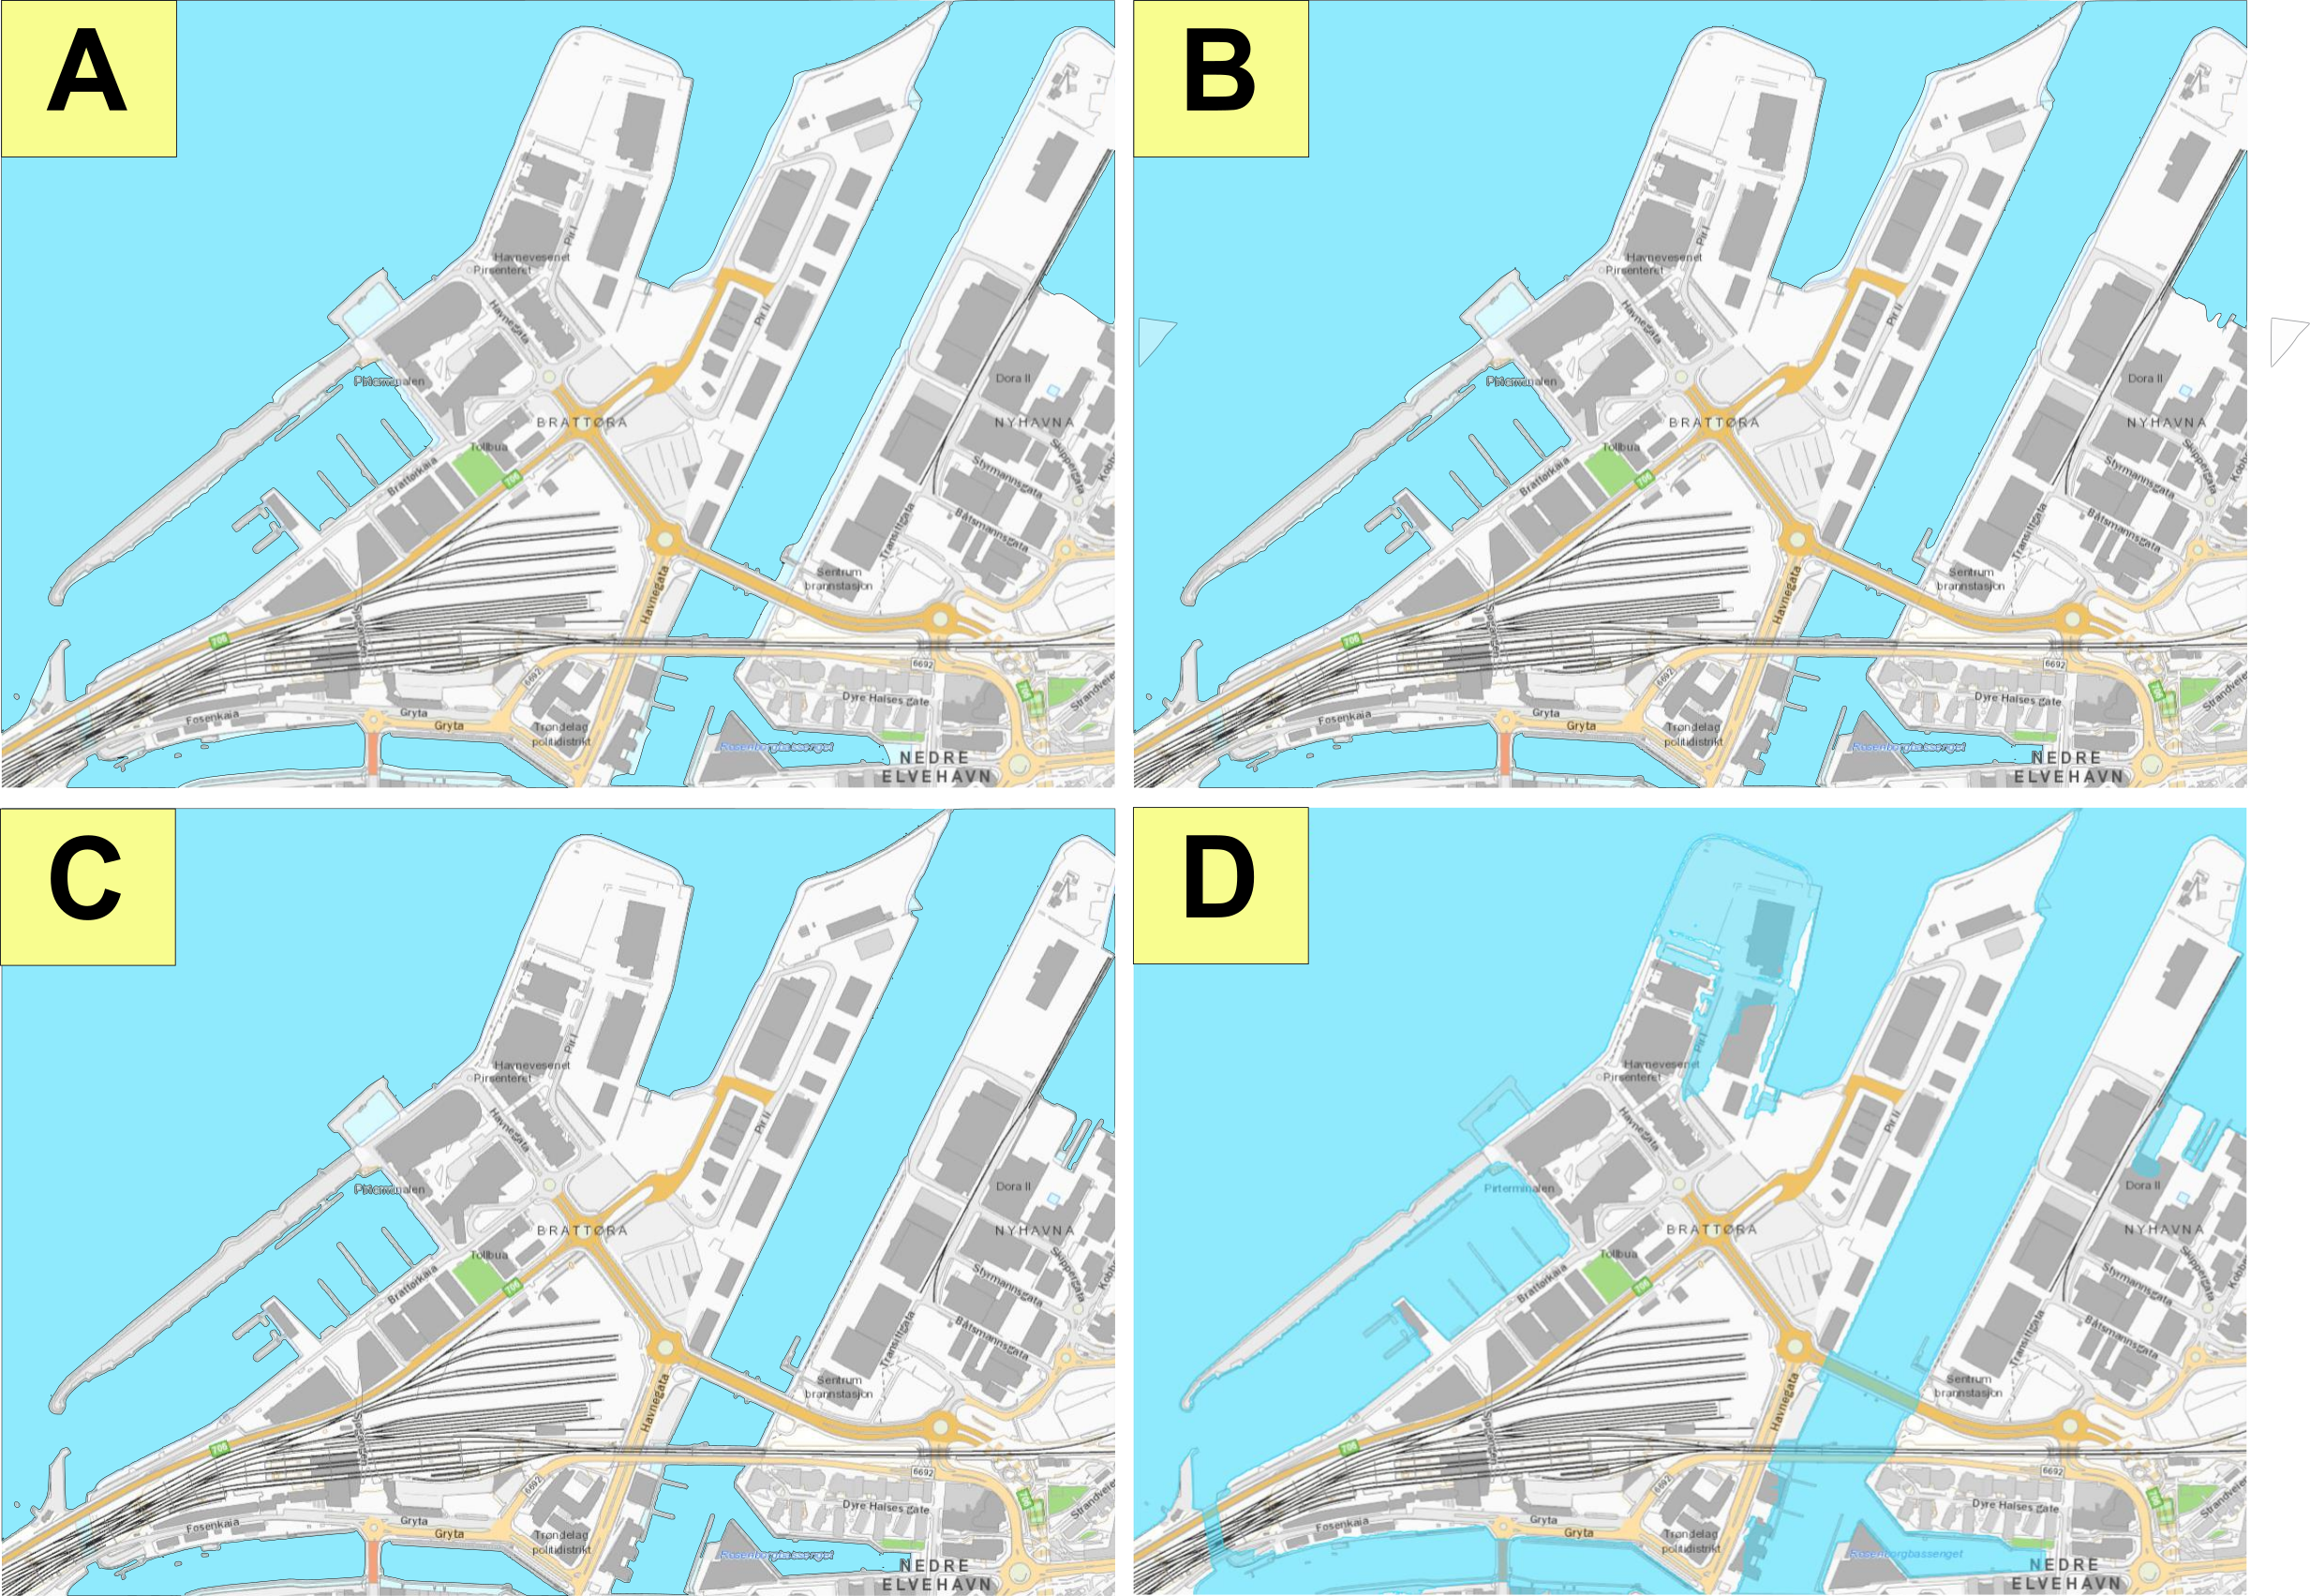
\includegraphics[width=16cm]{fig/brattora question on 2022 high tide quadrant.png}
    \caption{Which image displays Brattøra's High tide? -  This image contains four maps representing potential high tides in Brattøra. The map which matched models from \cite{kartverket_se_2021} is C. If subjects selected this response they were deemed aware of high tide in this place in the period 2022 to 2050. }
    \label{fig:Brattora_2022_hightide}
\end{figure}

\begin{figure}[H]
    \centering
    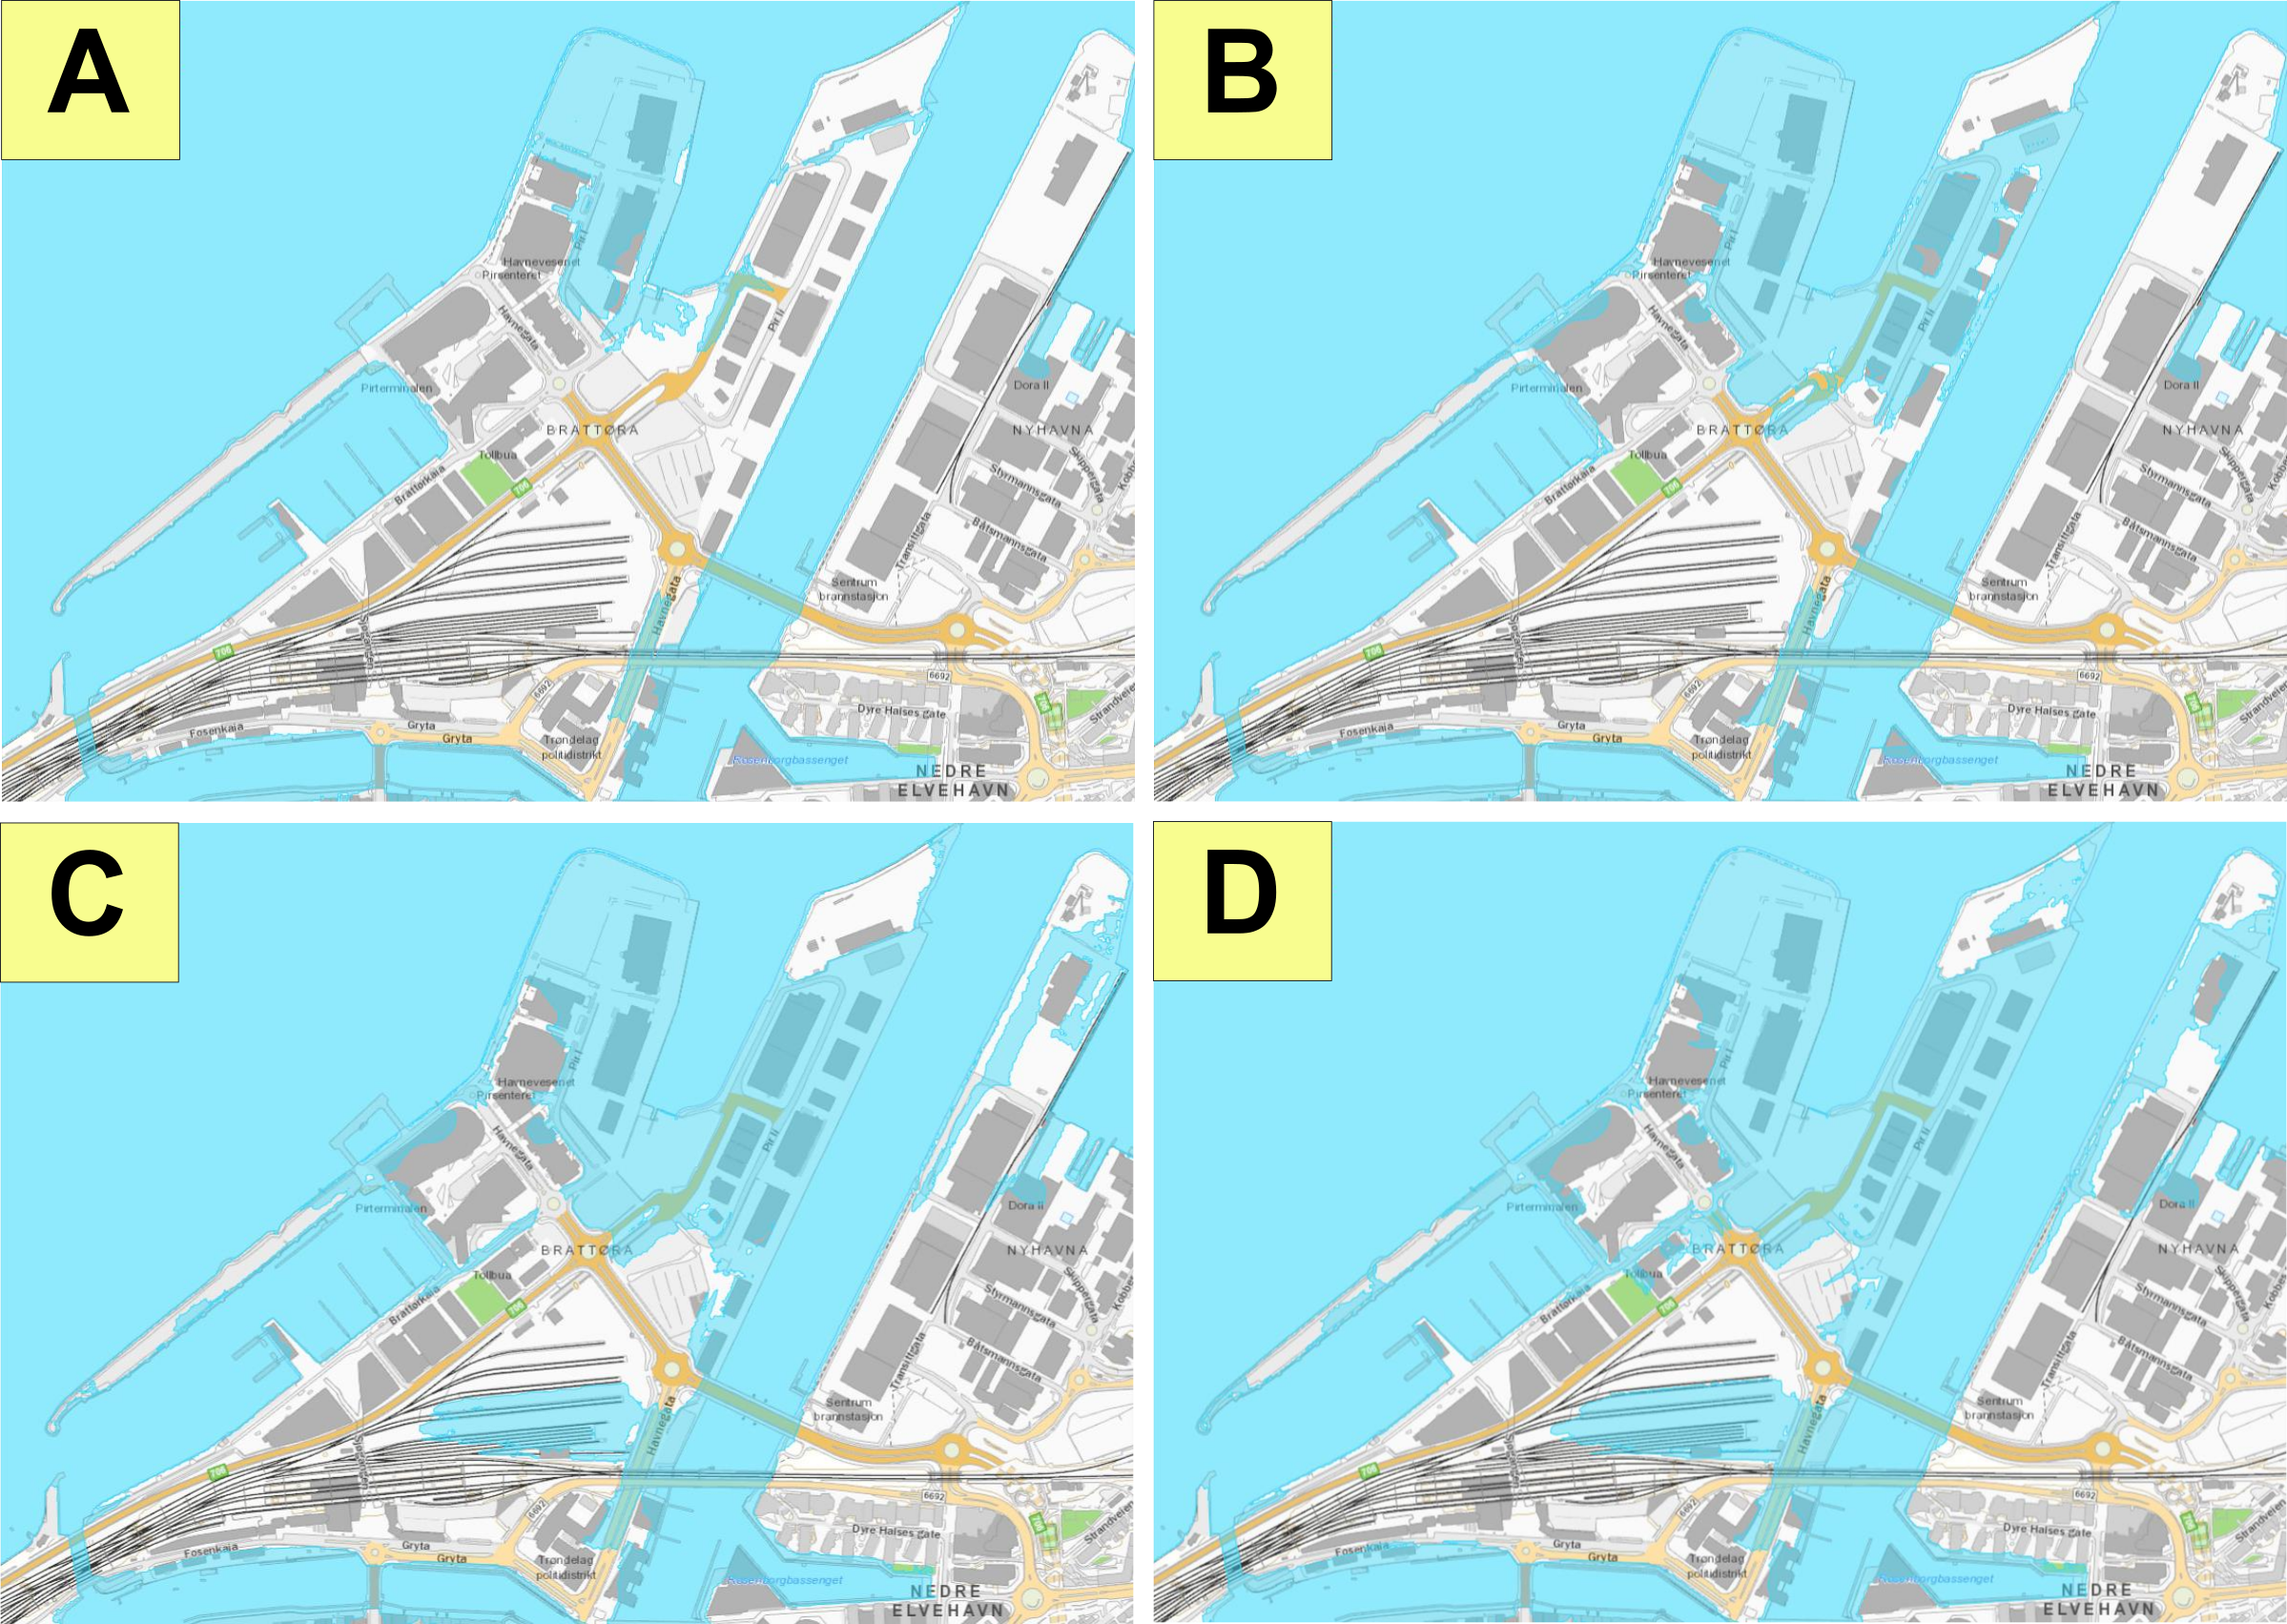
\includegraphics[width=16cm]{fig/brattora question on 2090 20 yr storm surge quadrant.png} 
    \caption{Which image displays Brattøra's 20 year storm surge in 2090? - This image contains four maps representing potential heights which could be caused by the 20 year storm surge. The map which matched the models from \cite{kartverket_se_2021} is B.If subjects chose this response they were deemed aware of the 20 year storm surge in the period 2050 to 2100. }
    \label{fig:brattora_2090_stormsurge}
\end{figure}

\begin{figure}[H]
    \centering
    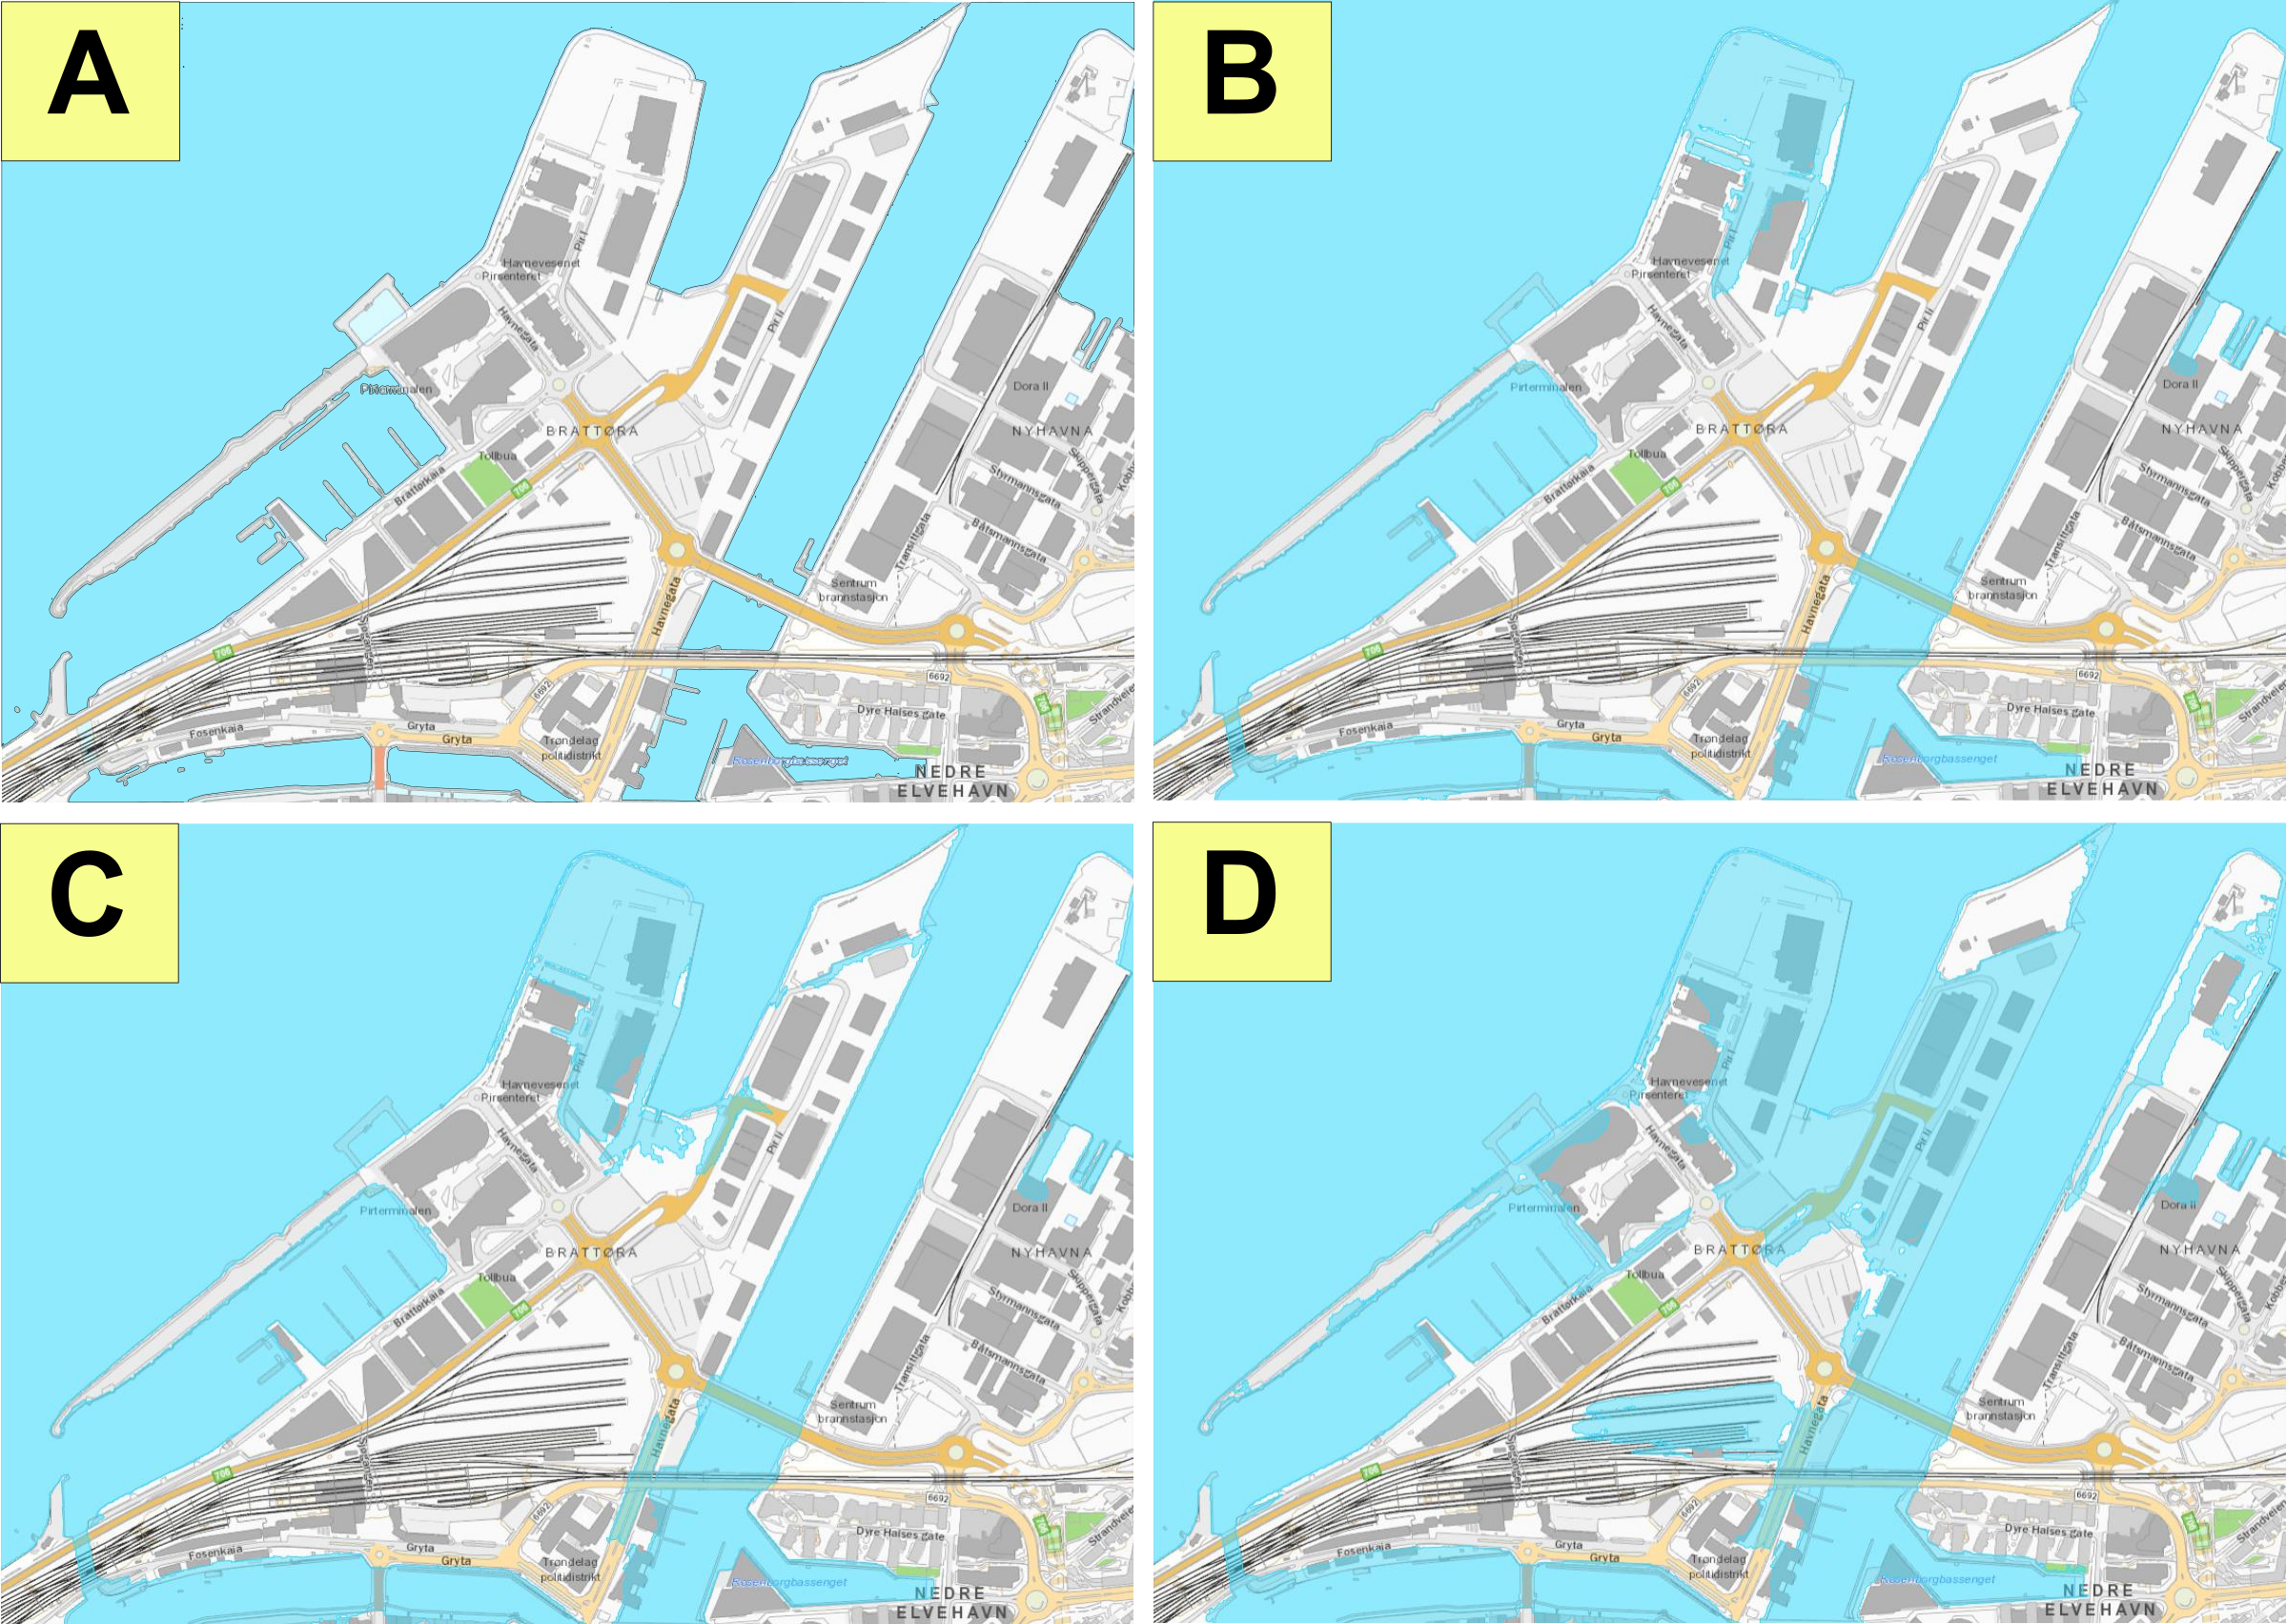
\includegraphics[width=16cm]{fig/brattora question on 2022 20 yr storm surge quadrant.png}
    \caption{Which image displays Brattøra's 20 year storm surge in 2022? - This image contains four maps representing potential heights which could be caused by the 20 year storm surge. The map which matched the models from \cite{kartverket_se_2021} is B.If subjects chose this response they were deemed aware of the 20 year storm surge in the period 2022 to 2050.}
    \label{fig:brattora_2022_stormsurge}
\end{figure}

The difficulty the participants had answering these questions is discussed in the results. After this, a focus group was conducted with seven of the subjects from the pilot survey.  They were shown Figure 3.4, which was used to direct conversation. The purpose of the focus group was to determine whether the subjects truly had high levels of awareness about SLEs and if so, what prevented them from choosing the correct answers. The findings from the pilot survey and focus group were used to improve data collection methods. 

\begin{figure}[H]
    \centering
    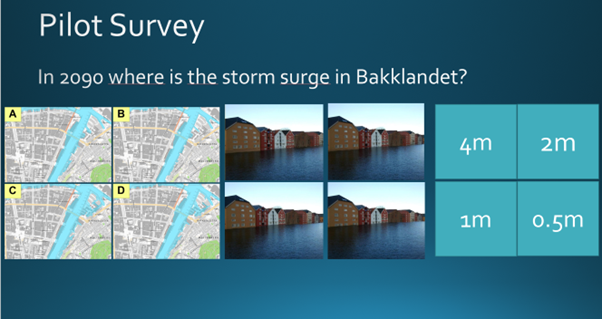
\includegraphics[width=1\textwidth]{fig_results/slide-pilot-survey.png}
    \caption{Image shown as part of focus group}
    \label{fig:slide}
\end{figure}

\section{Digital Visualisation of SLEs}
To determine Trondheim's social resilience, a survey was carried out in the summer of 2022. A key aim of this survey was to determine subjects' awareness of changing SLEs.  Five questions were asked to gauge awareness. Three questions utilised visual simulations of SLEs for each of the research sites. These were created based on models from \cite{dsb_integrating-sea-level-rise-and-storm-surges--local-planningpdf_2017} and \cite{kartverket_se_2020}. Images were created for various potential SLEs at the chosen research sites. Photographs of the sites were taken to make understanding and editing as easy as possible. They were taken on a sunny day, minimising people and boats, while attempting to capture recognisable landmarks. The geo-location and timing of the photos were noted to allow for determination of the water height. Table 3.1 below displays the water height of each of the original photographs. 
\paragraph{}

\begin{table}[h!]
    \centering
    \begin{tabular}{|l|l|}
        \hline
     	\textbf{Research Site} & \textbf{Photograph water level (cm)} \\ \hline
            Grillstad & 50 \\ \hline
            Skansen & -23 \\ \hline
            Nidelva & -159 \\ \hline
            Brattøra	& -42 \\ \hline
    \end{tabular}
    \caption{Water levels on day of photo taken for simulated SLEs this was determined from \cite{tides_high_2022}. Water levels included consideration of tide plus weather effects plus river levels}
    \label{tab:water_level_photo}
\end{table}
\paragraph{}

Using \cite{tides_high_2022} the base water level for each of the original photographs was determined. For Skansen, Grillstad and Brattøra, this meant combining the tides, plus weather effects. On most days, a calculation of Nidelva research site's water level would need to include the river level. However, time and day chosen was one with an observably low river level which allowed for this value to be excluded as water level was dominated by the tide at the time of the photo being taken.   
\paragraph{}

To these base water level photographs the simulated water levels could be digitally added. See the results Chapter for images. Table 3.2 and 3.3 below show the SLEs and the associated water level with NN2000 as a reference point.  To be able to accurately add the simulated water levels to the images, the first step is to make sure that each of the photos included a reference height. These key features (bins, fences, permanent benches, windows) were measured using a tape measure to allow for simulated realignment of the water levels to particular heights. Perspective was an important consideration in the original photos. Having the coastline at an angle allowed for a more realistic image, but did complicate the photo editing. 

\begin{table}[h!]
    \centering
    \begin{tabular}{|l|l|l|l|l|l|}
    \hline
     Sea Level &   mean high  & mean high  & 20 year  & 200 year   & 1000 year  \\ \newline
     Extreme &  water neaps & water springs &  storm surge  & storm surge  &  storm surge  \\ \hline
       Height (cm) &  55 & 119 & 216 & 234 & 244 \\ \hline
    \end{tabular}
    \caption{2022 SLEs Projections \cite{kartverket_se_2020}}
    \label{2022_sle_projections}
\end{table}

\begin{table}[h!]
    \centering
    \begin{tabular}{|l|l|l|l|l|}
    \hline
       Sea Level &  mean high & 20 year   & 200 year &  1000 year   \\ \newline
       Extreme & water springs &  storm surge  &  storm surge  &  storm surge  \\ \hline
       Height (cm) & 172 & 269 & 286 & 297 \\ \hline
    \end{tabular}
    \caption{2090 SLEs Projections \cite{kartverket_se_2020}}
    \label{2090_sle_projections}
\end{table}

Once the heights were calculated from the tables above, they were drawn onto the original photos using Inkscape. This new image was then used as the base layer when simulating SLEs. The original image was replicated twice using GIMP, GNU Image Manipulation Program, with a reduced opacity. The extra layer allowed for easier fixes during the next step. 
\paragraph{}
The top layer was then cut to leave only the water present in the image using the free select tool. If too much was cut the layer underneath could be used as a back up. After this, the handle transformation tool was used to define points. This layer was then aligned for each of the draw-upon water levels. Soft eraser tool was used to minimise oddities in the water created due to this movement. Dodge tool was used to darken below the water line to make the water line more distinct, as calm bright days were chosen, meaning the edge of the water was difficult to pin point on small screens. Finally, the clone tool was used to remove potential distractions, including seagulls and boats floating on the sea. The image was then exported as a JPEG. 

\paragraph{}
The final values and water levels used were rounded to 10cm for ease. The exported JPEGs were combined into grids and labelled for use in the survey. 

\section{Stakeholder Selection}
A subject's identity is a key part of the research. The nature of stakeholder participation during this project was limited to communication and consultation according to Rowe and Frower  (Rowe and Frower 2000 in \cite{reed_stakeholder_2008}). These stakeholders were selected in a predominately top down manner:  certain communities were targeted and individuals within these communities were asked to self identify (\cite{reed_stakeholder_2008}). However, there was also bottom up stakeholder identification as subjects could write in which communities they felt part of, beyond those decided on during the project design (\cite{reed_stakeholder_2008}). An understanding of what and who the stakeholders are in the changing impacts of SLEs in Trondheim was essential to allow the assessment of local knowledge and awareness. However stakeholder theory is not used as an analytical method.
\paragraph{}
The results will be published in an accessible form for those stakeholders who are interested. This is in line with the guidelines for citizen science set out by \cite{tweddle_guide_2012}. The data management plan and ethics guidance were created in line with \cite{nesh_guidelines_2022} and \cite{nsd_norsk_nodate}. 

\section{Data Analysis of Survey Results}
An exploratory data analysis was completed then non parametric hypothesis testing was conducted utilising RStudio. Histograms and Shapiro Tests were used to determine the distribution and scatter-plots were created to search for linear relationships. The results of the analysis were exported from R Studio to Microsoft Excel for ease of plotting.
\paragraph{}
The main survey comprised of 26 questions addressing awareness, memory of SLEs, interest levels in SLEs, community membership, information access, length of residence, attitudes as well as space to highlight other place-based risks. Linear regression and linear mixed effect models were originally planned as the main statistical analyses, but due to the lack of linearity, highlighted by the scatterplots in the exploratory analysis, non-parametric hypothesis testing was selected.


However, due to lack of linearity in original scatter-plots another method was also chosen. 153 responses were collected. 30 percent of respondents had no memory of SLEs in Trondheim with 70 percent having memory of one or more event. A third (50/153) remembered the most recent sea level extreme in February 2020. 
\paragraph{}
A non parametric hypothesis testing method was chosen due to the lack of linearity, and as the data was not normally distributed. Specifically the Kruskal Wallis Rank Sum Test based off \cite{hollander_nonparametric_2014} due to the need to investigate multiple groups, upon one variable and having only measured each subject once. Both \cite{tasman_how_2014} and \cite{hollander_nonparametric_2014}, were consulted to make this decision. Logistic regression was considered, but was rejected as splitting awareness into a dummy variable would have been the most significant impact on the results. The survey data was collected via the online survey tool, Nettskjema, codified and then exported to RStudio, which was used to analyse all quantitative data.
\paragraph{}
Participant diversity is inherently biased when relying on goodwill, but a wide range of levels of interest in SLEs and community membership were surveyed including those who were not interested and who had limited knowledge of Trondheim’s coasts, as can be seen in the results. The original intention was to determine awareness as the ability to answer five questions. This would hopefully create a homoscedasticitic (i.e. the residuals have constant variance at every level of x) variable with independent and normally distributed residuals. However, quick analysis of the data showed that this would not be the case.
\paragraph{}
For example, only three subjects answered correctly to the question "How much do you think the sea level has changed in the past 30 years?", creating a skewed distribution. For this reason this variable has been excluded from the main determination of awareness. This does not mean it is not considered in the answer to research question 2, but research question 3 requires a significant percentage being deemed aware. 
\paragraph{}
A higher percentage answered correctly to the question "How much do you think the sea level will change in the next 30 years?". However, this percentage was deemed insignificant and more due to luck as 2/7 answers were appropriate. For this reason, this variable was also excluded for the determination of awareness as used to answer research question 3. However, it is used when answering research question 2. The other questions used to determine awareness utilised images with simulations of SLE's, unlike those questions which solely used numeric values. This is another reason why only three questions were included in the determination of awareness in contrast with the original plan. The exclusion of these variables is discussed later in this paper including differences around understanding gained from images or a number.
\paragraph{}
Awareness was calculated using the responses to the three questions "Which image shows the current 20-year storm surge?", "Which image shows the 20-year storm surge projected for 2090?" and "Which image displays the current high tide?". The full survey in both Norwegian and English is in the appendix. This shows how subjects received both numeric and visual representation of the SLEs when answering these questions. 



